\documentclass[intlimits, 9pt, unicode]{beamer} 

\usepackage[T2A]{fontenc}
%\usepackage[cp1251]{inputenc}
\usepackage[utf8]{inputenc}
\usepackage[russian]{babel}
\usepackage{graphicx}
\usepackage{amssymb}
\usepackage{amsthm}

\usefonttheme[onlymath]{serif}

\usepackage{beamerthemesplit}

\usetheme{Warsaw}

\setbeamerfont{institute}{size=\normalsize}

\setbeamercolor{bluetext_color}{fg=blue}
\newcommand{\bluetext}[1]{{\usebeamercolor[fg]{bluetext_color}#1}}

\setbeamercovered{transparent}

\title{Change point detection in mobile advertising}
\author{Nina Golyandina, Kliment Merzlyakov}
\institute{Saint Petersburg State University \\
    Mathematical faculty \\
     Applied statistics department \\
}
\date{
    Saint Petersburg\\
    2018
}

\begin{document}

\begin{frame}
    \titlepage
\end{frame}

\begin{frame}
    \frametitle{Content}

    \begin{itemize}
    	\item Change point detection
		     	 \begin{itemize}
	    		   \item What is change point detection
		    	   \item Real world examples of change point detection 
		    	   \item Reasons to detect change points
		    	  \end{itemize}
        \item Change point detection techniques
        \item Airpush cases
		     	 \begin{itemize}
	    		   \item Fraud elimination
		    	   \item Trend extraction
		    	   \item Smart alerts
		    	  \end{itemize}
    \end{itemize}
\end{frame}


\begin{frame}
    \frametitle{Change point detection}

    \begin{itemize}
    	\item Change point --- point in time series where some significant change occured
	\item Change point detection --- group of methods to find change points in time series
    \end{itemize}
\end{frame}

\begin{frame}
    \frametitle{Types of change points}

    \begin{itemize}
    	\item Trend change
	\item Mean change
	\item Variance change
	\item Single point change
	\item Period change
    \end{itemize}
\end{frame}

\begin{frame}
\frametitle{Pictures}
\begin{figure}
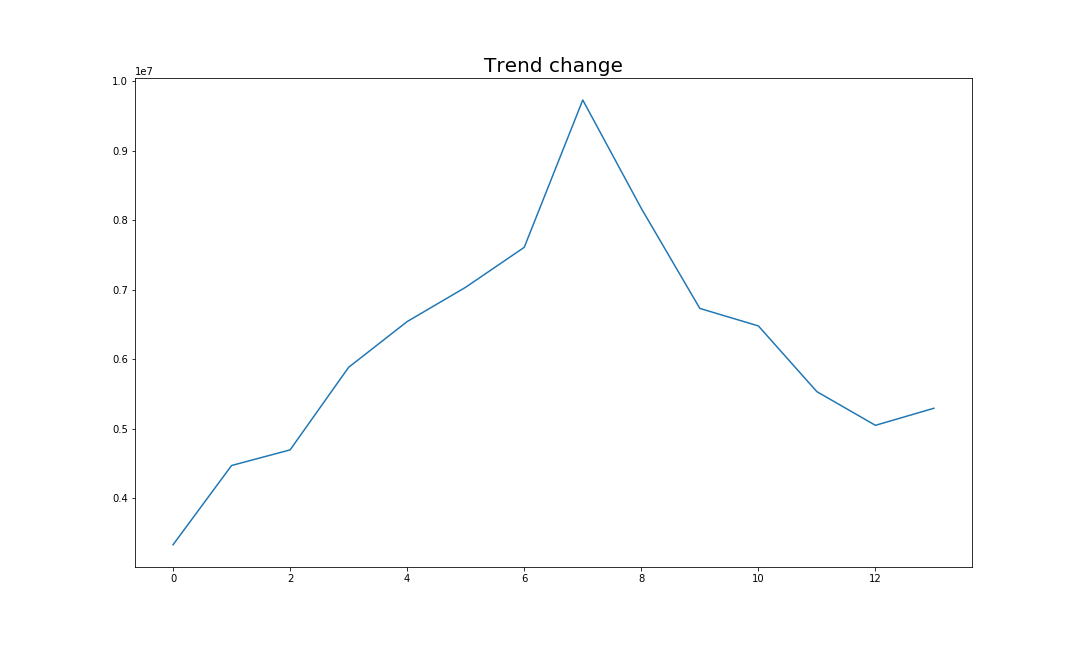
\includegraphics[scale=0.30]{images/001_trend_change}
\end{figure}
\end{frame}


\end{document}
